% Direct Form II biquad — DSP signal-flow graph
% Compile:  pdflatex biquad-df2-signal-flow.tex            -> PDF
%           dvisvgm --pdf --no-fonts biquad-df2-signal-flow.pdf   -> editable SVG (text as vector paths)
% or keep text editable:  dvisvgm --pdf --font-format=woff biquad-df2-signal-flow.pdf
\documentclass[border=6pt]{standalone}
\usepackage{amsmath}
\usepackage{tikz}
\usetikzlibrary{shapes.geometric, arrows.meta, positioning, calc}

% ---- reusable signal-flow styles -------------------------------------------
\tikzset{
  >={Stealth[length=2.4mm]},
  wire/.style={line width=0.7pt},
  adder/.style={circle, draw, line width=0.7pt, minimum size=6mm, inner sep=0pt},
  gainf/.style={% feed-forward gain, apex points right
    isosceles triangle, draw, line width=0.7pt,
    isosceles triangle apex angle=55, minimum width=9mm, inner sep=2pt},
  gainb/.style={% feed-back gain, apex points left
    gainf, shape border rotate=180},
  delay/.style={rectangle, draw, line width=0.7pt, minimum size=8mm, inner sep=2pt},
  tap/.style={circle, fill, minimum size=3.4pt, inner sep=0pt},
}

\begin{document}
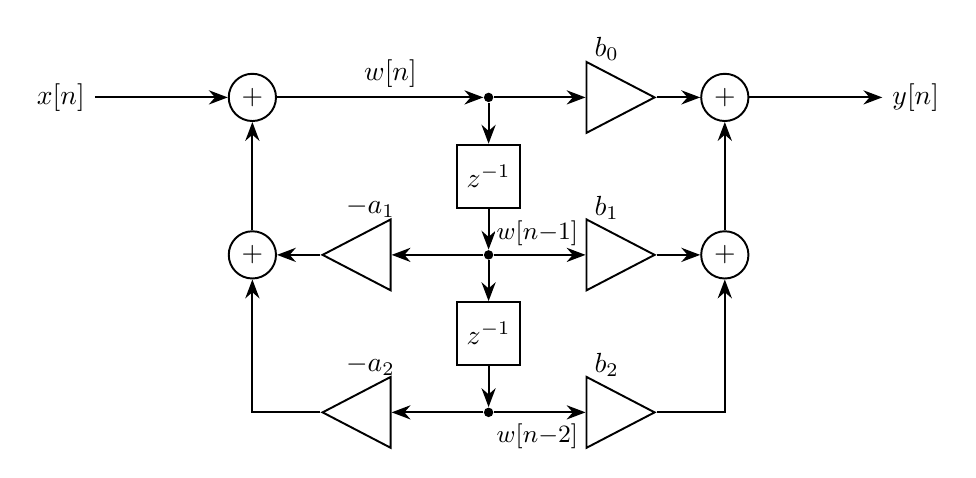
\begin{tikzpicture}[node distance=0pt]

  % ----- core nodes ---------------------------------------------------------
  \node[adder] (sin)  at (0,0)  {$+$};      % input summing node
  \node[tap]   (c0)   at (3,0)  {};         % w[n]
  \node[delay] (d1)   at (3,-1) {$z^{-1}$};
  \node[tap]   (c1)   at (3,-2) {};         % w[n-1]
  \node[delay] (d2)   at (3,-3) {$z^{-1}$};
  \node[tap]   (c2)   at (3,-4) {};         % w[n-2]

  \node[adder] (sout) at (6,0)  {$+$};      % output summing node (top)
  \node[adder] (pf)   at (6,-2) {$+$};      % feed-forward partial sum

  \node[adder] (qb)   at (0,-2) {$+$};      % feed-back partial sum

  % ----- gain triangles -----------------------------------------------------
  \node[gainf] (b0) at (4.5,0)  {};   \node at (4.5,0.62) {$b_0$};
  \node[gainf] (b1) at (4.5,-2) {};   \node at (4.5,-1.4) {$b_1$};
  \node[gainf] (b2) at (4.5,-4) {};   \node at (4.5,-3.4) {$b_2$};
  \node[gainb] (a1) at (1.5,-2) {};   \node at (1.5,-1.4) {$-a_1$};
  \node[gainb] (a2) at (1.5,-4) {};   \node at (1.5,-3.4) {$-a_2$};

  % ----- central delay line -------------------------------------------------
  \draw[wire,->] (sin) -- node[above,pos=0.55]{$w[n]$} (c0);
  \draw[wire,->] (c0) -- (d1);
  \draw[wire,->] (d1) -- (c1);
  \draw[wire,->] (c1) -- (d2);
  \draw[wire,->] (d2) -- (c2);
  \node[fill=white, inner sep=0.6pt] at (3.62,-1.72) {\small$w[n{-}1]$};
  \node[fill=white, inner sep=0.6pt] at (3.62,-4.30) {\small$w[n{-}2]$};

  % ----- input / output ports ----------------------------------------------
  \draw[wire,->] (-2,0) node[left]{$x[n]$} -- (sin);
  \draw[wire,->] (sout) -- (8,0) node[right]{$y[n]$};

  % ----- feed-forward paths (taps -> gains -> adders) -----------------------
  \draw[wire,->] (c0) -- (b0.west);
  \draw[wire,->] (b0.east) -- (sout.west);
  \draw[wire,->] (c1) -- (b1.west);
  \draw[wire,->] (b1.east) -- (pf.west);
  \draw[wire,->] (c2) -- (b2.west);
  \draw[wire,->] (b2.east) -| (pf.south);
  \draw[wire,->] (pf.north) -- (sout.south);

  % ----- feed-back paths (taps -> gains -> input adder) ---------------------
  \draw[wire,->] (c1) -- (a1.east);
  \draw[wire,->] (a1.west) -- (qb.east);
  \draw[wire,->] (c2) -- (a2.east);
  \draw[wire,->] (a2.west) -| (qb.south);
  \draw[wire,->] (qb.north) -- (sin.south);

\end{tikzpicture}
\end{document}
